\label{sec:implementation}

\doubletake{} is implemented as a library and can be linked directly to programs, or can be injected into unmodified binaries by setting the \texttt{LD\_PRELOAD} environment variable on Linux.

At startup, \doubletake{} begins a new epoch. The epoch continues until the program issues an \emph{irrevocable} system call (see Section~\ref{sec:syscalls} for details). Before this call is issued, \doubletake{} scans program state for evidence of errors. The details of this scan are presented in Section~\ref{sec:applications}.

If no errors are found \doubletake{} ends the epoch, issues the irrevocable system call, and begins a new epoch. If any detection tools have found evidence of an error, \doubletake{} enters re-execution mode. The remainder of this section describes the implementation of \doubletake{}'s core functionality.

\subsection{Epoch Start}
\label{sec:implementation/start}

At the beginning of each epoch, \doubletake{} takes a snapshot of program state. \doubletake{} saves all writable memory (stack, heap, and globals) from the main program and any linked libraries, and saves register state of each thread with the \texttt{getcontext} function. Read-only memory does not need to be saved. To identify all writable mapped memory, \doubletake{} reads the Linux \texttt{/proc/self/map} file. \doubletake{} also saves file positions of all open files. This lets programs issue \texttt{read} and \texttt{write} system calls without ending the current epoch. \doubletake{} uses the saved memory state and file offset to ``undo'' these calls if the epoch needs to be re-executed when an error is found.

%%%%%%%%%%%%%%%%%%%%%%%%%%%

\subsection{Normal Execution}
\label{sec:implementation/normalexecution}

Once a snapshot has been saved, \doubletake{} lets the program execute normally. Most program operations proceed normally, but \doubletake{} interposes on heap allocations and system calls in order to set tripwires and support re-execution.

%%%%%%%%%%%%%%

\subsubsection*{System Calls}
\label{sec:syscalls}
\begin{table}[t]
	\centering
	\small
	\renewcommand{\arraystretch}{1.5}
	\begin{tabular}{l|p{6cm}}
		\textbf{Category} & \textbf{Functions} \\
		\hline
		
		Repeatable		& \texttt{getpid}, \texttt{sleep}, \texttt{pause}\\
		
		Recordable		& \texttt{mmap}, \texttt{gettimeofday}, \texttt{time}, 
						  \texttt{clone} , \texttt{open}\\
		
		Revocable		& \texttt{write}, \texttt{read} \\
		
		Deferrable		& \texttt{close}, \texttt{munmap} \\
		
		Irrevocable		& \texttt{fork}, \texttt{exec}, \texttt{exit}, \texttt{lseek}, \texttt{pipe}, \texttt{flock}, \texttt{socket related system calls}\\
	\end{tabular}
	\caption{System calls handled by \doubletake{}. All unlisted system calls are conservatively treated as irrevocable, and will end the current epoch. Section~\ref{sec:syscalls} describes how \doubletake{} handles calls in each category.\label{table:syscalls}}
\end{table}

\doubletake{} ends each epoch when the program attempts to issue an irrevocable system call. However, most system calls can safely be re-executed or undone prior to re-execution. 

\doubletake{} breaks system calls into five categories, shown in Table~\ref{table:syscalls}. System calls could be intercepted using \texttt{ptrace}, but this would add unacceptable overhead during normal execution. Instead, \doubletake{} interposes on all library functions that may issue system calls.

%%%%%%%

\emph{Repeatable system calls} do not modify system state, and return the same result during normal execution and re-execution. No special handling is required for these calls.

\begin{figure*}[ht!]
	\begin{center}
		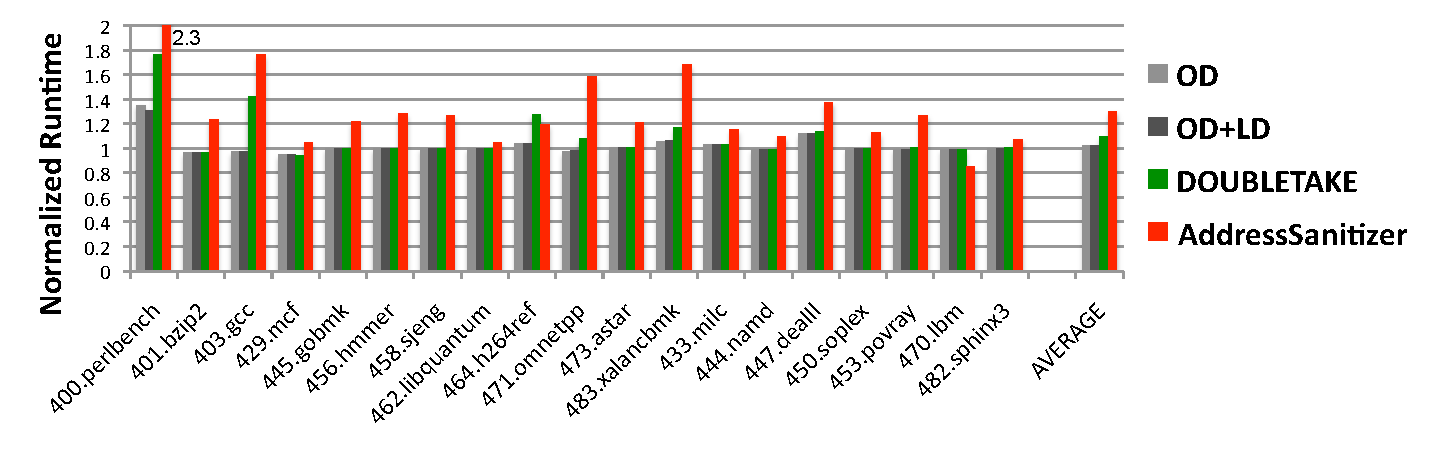
\includegraphics[width=6.5in]{figure/perf}
	\end{center}
	\caption{Runtime overhead of \doubletake{} (OD = Buffer Overflow Detection, LD = Leak Detection, \doubletake{} = all three detections enabled) and AddressSanitizer, normalized to each benchmark's original execution time. 
%Overhead for Valgrind is reported in Table~\ref{table:valgrind} because the results do not fit on this graph.
\label{fig:perf}}
\end{figure*}

%%%%%%%

\emph{Recordable system calls} may return different results if they are re-executed. \doubletake{} records the result of these system calls during normal execution, and returns the saved result during re-execution. Some recordable system calls, such as \texttt{mmap}, change the state of underlying operating system. Memory mapped with a call to \texttt{mmap} is left mapped for the entire epoch's re-execution; this is safe because the program cannot access this memory until the point at which the \texttt{mmap} call is replayed.

\emph{Revocable system calls} modify system state, but \doubletake{} can save the original state beforehand and restore it prior to re-execution. Most file I/O fall into this category.

For example, \texttt{write} modifies file contents, \doubletake{} can write the same content during re-execution. \texttt{write} also changes the current file position, which \doubletake{} restores to the saved file position using \texttt{lseek} prior to re-execution. \doubletake{} saves all file descriptors of opened files in a hash table at the beginning of each epoch. In addition, \doubletake{} must save stream contents returned by \texttt{fread}. Calls to \texttt{read} and \texttt{write}  on normal files, which can be identified by check the hash map, don't need to be handled. But those calls on socket files are treated as irrevocable system calls.
	
\emph{Deferrable system calls} will irrevocably change program state, but can safely be delayed until the end of the current epoch. \doubletake{} delays all calls to \texttt{munmap} and \texttt{close}, and executes these system calls before exiting or starting a new epoch.
	
\emph{Irrevocable system calls} change internally-visible program state, and cannot be undone. \doubletake{} must end the current epoch before these system calls are allowed to proceed. Note that for \doubletake{}, the meaning of ``irrevocable'' is different from that used in transactional memory systems~\cite{Irrevocabletrans}. Unlike in transactions, we expect re-execution to be identical to the epoch's original execution. It is safe for system calls to affect externally-visible state as long as the effect on internal state can be hidden or undone.

Note that in the presence of multiple threads, an error may fail to appear in the re-execution because of data races (synchronization ordering is already tracked and replayed). \doubletake{} then re-executes the code in an attempt to reveal the error. If it fails to reveal the error on replay, \doubletake{} has effectively tolerated the error and continues execution.

%%%%%%%%%%%%%%

\subsubsection*{Multithreaded Support}
We have implemented support for multiple threads, but the recording and re-execution of thread synchronizations is not yet stable. \doubletake{} records the sequence of system calls and results separately for each thread.

Every mutex records the order of threads that acquire it, and condition variables record the order of thread wakeups. \doubletake{} does not enforce a total global order on lock acquisitions. Operations within a single thread are totally-ordered, and \doubletake{} enforces local order at each synchronization point. In the absence of data races, this is sufficient to ensure deterministic re-execution.

Calls to \texttt{pthread\_create} are recorded with the same mechanism as recordable system calls. When a new thread starts, \doubletake{} takes a snapshot of the thread's stack and registers to enable re-execution from the beginning of the thread's execution. As with synchronization operations, \doubletake{} logs thread creation order and enforces this order during re-execution. Calls to \texttt{pthread\_exit} are deferred until the end of the epoch. Because \texttt{pthread\_exit} is deferred, \texttt{pthread\_join} is effectively deferred as well.

%%%%%%%%%%%%%%

\subsubsection*{Heap Allocator}
\label{sec:heapallocator}

Heap allocators typically issue a large number of \texttt{mmap} or \texttt{sbrk} system calls, which would complicate \doubletake{}'s logging re-execution. \doubletake{} replaces the default heap with a fixed-size BiBOP-style allocator with per-thread subheaps and power-of-two size classes, built using Heap Layers~\cite{heaplayers}. \doubletake{}'s heap is completely deterministic, so no logging is required to ensure that allocations do not change during re-execution.

When an object is freed, the allocator checks which subheap it is allocated from. If the object comes from the freeing thread's subheap, the \texttt{free} call proceeds uninterrupted. If the object was originally allocated by a different thread, the \texttt{free} is deferred. When the epoch ends, each object whose \texttt{free} was deferred is returned to its source thread's freelist.

During replay, \doubletake{}'s heap allocator checks to see if the object being allocated or freed contains the address where an error was detected. If so, \doubletake{} calls the \texttt{backtrace()} function to obtain a call stack for the allocation and deallocation sites.

\doubletake{} lets error detection tools traverse the set of all allocated objects during error checking. Objects are marked as allocated in object headers, including a size of the \emph{requested size}, which may be less than the power-of-two size class for object. All three detection tools use this size during scanning.

\doubletake{} also maintains a bitmap to record the locations of heap canaries. The bitmap records every word of heap memory that contains a canary. \doubletake{} notifies the detection tool when any of the bytes do not contain canaries. Buffer overflow detection places canaries only outside the requested object size. Re-execution is only started if the detection tool finds that canaries between allocated objects have been overwritten.

%%%%%%%%%%%%%%

\subsubsection*{Epoch End}

The epoch ends when any thread issues an irrevocable system call. All other threads are notified with a signal. Once all threads have stopped, \doubletake{} checks the program state for errors. The application-specific error checks are described in Section~\ref{sec:applications}. If an error is found, \doubletake{} immediately switches to re-execution mode. If not, the runtime issues any deferred system calls and clears the logs for all recorded system calls.

%%%%%%%%%%%%%%%%%%%%%%%%%%%

\subsection{Re-Execution}
\label{sec:implementation/re-execution}

Before re-executing the current epoch, \doubletake{} must roll back program state. Restoring saved memory will overwrite the current stack, so \doubletake{} switches to a temporary stack during rollback. The saved state of all writable memory is copied back, and any revocable system calls are undone (see Section~\ref{sec:implementation/normalexecution} for details). Before restoring register state, \doubletake{} must allow detection tools to place watchpoints.

\subsubsection*{Watchpoints}
Debug registers are not accessible in user-mode, so \doubletake{} must use \texttt{ptrace} to set watchpoints. \doubletake{} forks a child process and attaches to it using \texttt{ptrace} to load watched addresses into the debug registers and enable the watchpoints.

Once watchpoints have been placed, \doubletake{} uses the \texttt{setcontext} call to restore register state and begin re-execution. During re-execution, \doubletake{} replays the saved results of system calls from the log collected during normal execution. All deferred system calls are converted to no-ops while the program is re-executing.

\subsection*{Synchronization Replay}
\doubletake{} enforces the recorded order of synchronization operations during re-execution. A thread can only acquire a mutex if it is the next thread in the acquisition log, regardless of whether the mutex is currently locked. \doubletake{} uses semaphores to wake threads from condition variables in the recorded order. When a condition variable is signaled, the signaling thread notifies next waking thread that it can resume. If this thread has not yet arrived at the condition variable, it will wake immediately after it arrives.
